% !TeX spellcheck = ru_RU
% !TEX root=../main.tex

\begin{lecture}[Супрамолекулярная сольватация]
\begin{lecSection}[Кавитанты]

\subsection{1. Кукурбитурил}

	\begin{figure}[H]

		\centering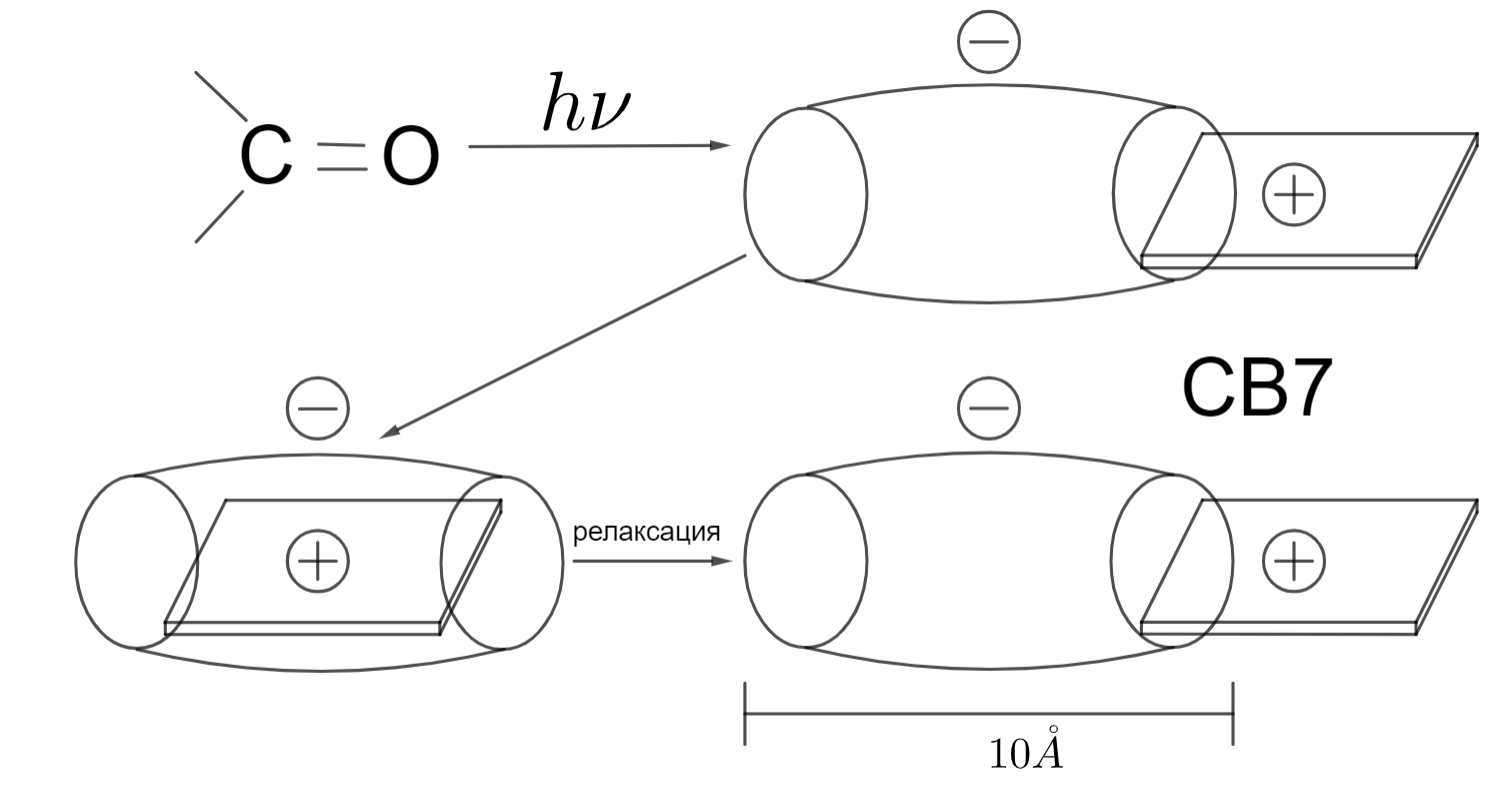
\includegraphics[width=0.9\linewidth]{lecture_09/pic1}
	
\end{figure}

$Kp + CB7 \rightleftharpoons Kp \subset CB7$ - комплексные включения.
\par $K = \dfrac{\left[ Kp \subset CB7 \right]}{[Kp][CB7]}$   $K \simeq 10^6 \dfrac{\text{л}}{\text{моль}}$

	\begin{figure}[H]
	
	\centering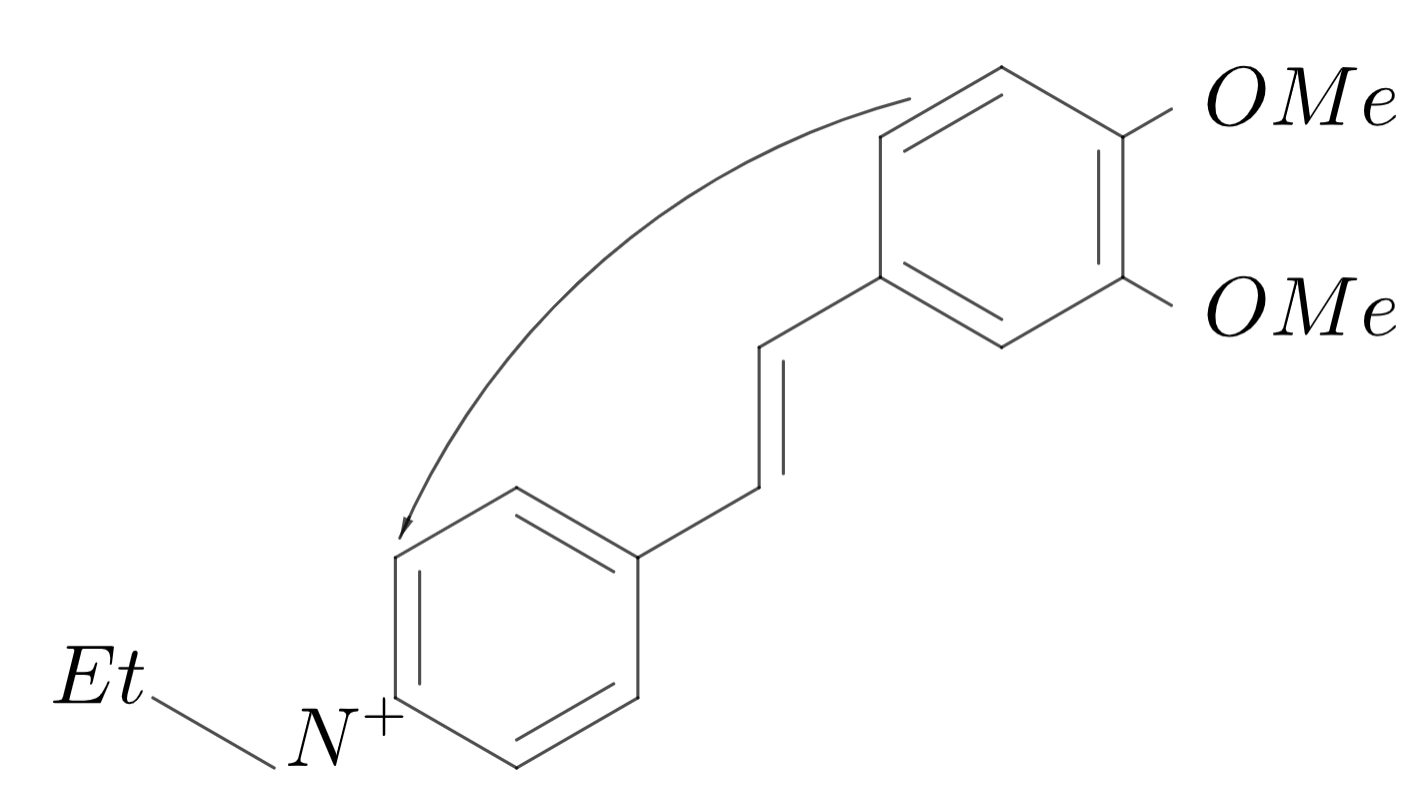
\includegraphics[width=0.6\linewidth]{lecture_09/pic2}
	
\end{figure}

\par Краситель, поглощает свет: $\lambda_ex = 400$ нм.
\par Получили молекулярную машину --- супрамолекулярную систему, в которой под действием внешнего стимула могут происходить существенные механические перемещения, и они должны происходить циклически. 

\subsection{2. Циклодекстрин}
	
		\begin{figure}[H]
		
		\centering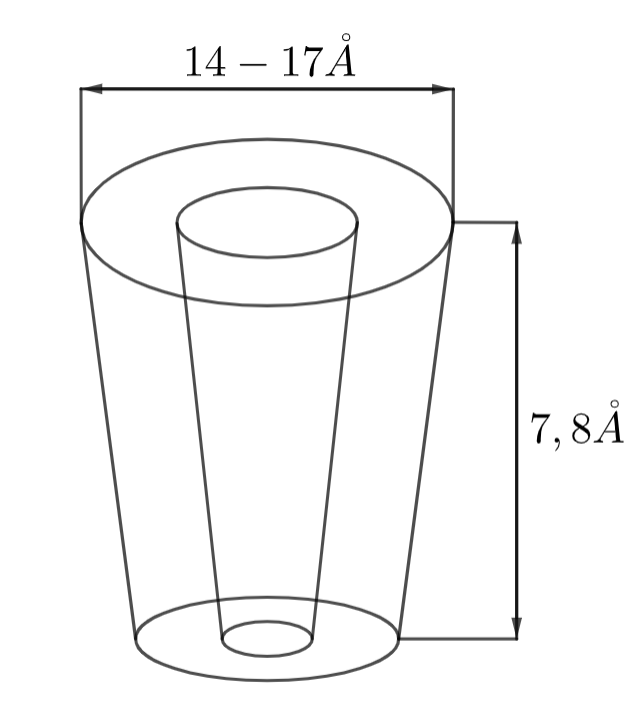
\includegraphics[width=0.6\linewidth]{lecture_09/pic3}
		
	\end{figure}

\par Используется в медицине. Полость гидрофобная, нижняя поверхность гидрофильная.

\subsection{2. Каликс[n]арены}

calix - чаша.

	\begin{figure}[H]
	\begin{minipage}[h]{0.49\linewidth}
		\centering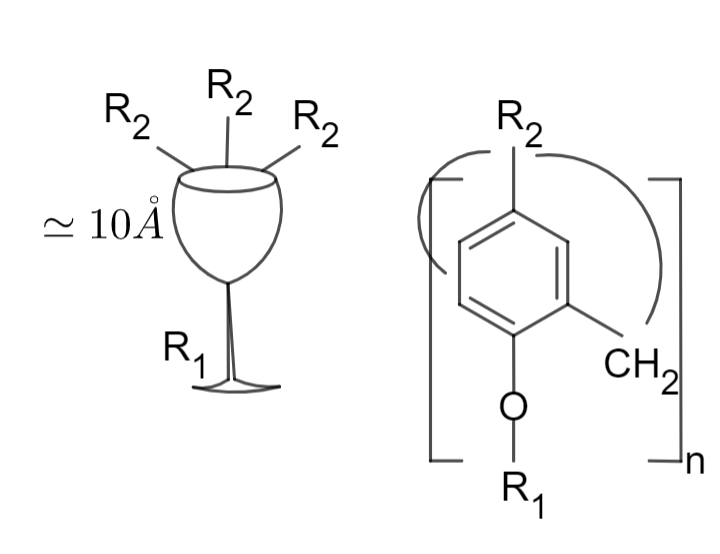
\includegraphics[width=\linewidth]{lecture_09/pic4}
		
	\end{minipage}
	\hfill
	\begin{minipage}[h]{0.49\linewidth}
		\centering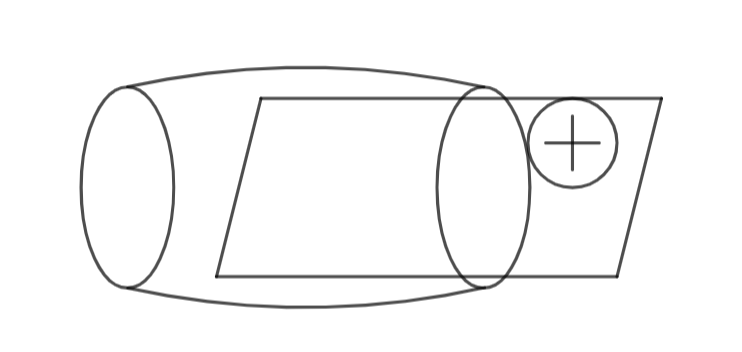
\includegraphics[width=\linewidth]{lecture_09/pic5}
	\end{minipage}
	
\end{figure}
	
\end{lecSection}

\begin{lecSection}[Селективная сольватация]
	
А/С - компоненты растворителя, $\varepsilon_A >> \varepsilon_C$

		\begin{figure}[H]
	
	\centering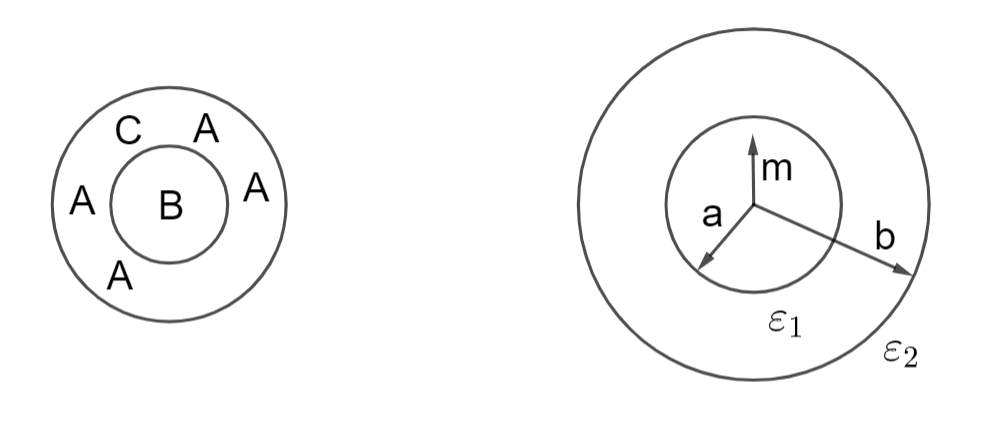
\includegraphics[width=\linewidth]{lecture_09/pic6}
	
\end{figure}	

Уравнение Лапласа: $\bigtriangleup \phi = 0$
$$\Phi = \dfrac{m cos \Theta}{r^2} - Rr cos \Theta, r < a$$
$$\Phi = \dfrac{Acos \Theta}{\varepsilon_1 r^2}, a < r < b$$
$$\Phi = \dfrac{Ccos \Theta}{\varepsilon_2 r^2}, r > b$$

\par Используем модель Онзагера
\par 1. $\phi$ - непреравная.
\par 2. $\varepsilon_1 \dfrac{\partial \phi}{\partial r} = \varepsilon_2 \dfrac{\partial \Phi}{\partial r}$
\par $\left(\dfrac{a}{b}\right)^3 = o(1)$
\par $R = \dfrac{2m}{a^3} \left(\dfrac{\varepsilon_1-1}{2 \varepsilon_1 + 1}\right) \left[1 + \dfrac{\varepsilon_2 - \varepsilon_1}{\varepsilon_1 + 2 \varepsilon_2} \cdot \dfrac{9 \varepsilon_1}{(\varepsilon_1 - 1)(1 + 2 \varepsilon_1)} \cdot \left( \dfrac{a}{b}\right)^3 \right]$
\par Ещё одно упрощение:
\par $\varepsilon_1 = 50, \varepsilon_2 = 5 \rightarrow R \simeq \dfrac{m}{a^3} \left[1 - \dfrac{9}{2a} \left(\dfrac{a}{b}\right)^3\right]$
\par $\Delta G = -mR$
\par Только ближайшее окружение в коненсированной фазе вносит основной вклад в сольватацию.

\par Борн: $\Delta G_s = - \dfrac{\varepsilon}{2a}(1-\varepsilon)$
\par Онзагер:$\Delta G_s = \dfrac{2m^2}{a} \left(
dfrac{\varepsilon - 1}{2 \varepsilon + 1}\right)$

	
\begin{figure}[H]
	
	\centering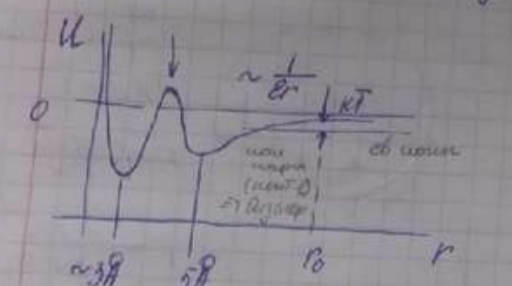
\includegraphics[width=0.6\linewidth]{lecture_09/pic7}
	
	\end{figure}
	
	\par Рассмотрели разбавленные системы.
	
\subsection{Дебай}

$\sim \dfrac{1}{r}$(определяет взаимодействие)
\par $U = \int_{d}^{\infty} U(r)dV \sim \int_{d}^{\infty} \dfrac{1}{r} 4 \pi r^2 dr$ - интеграл расходится на бесконечности. Предположили, что система однородно гомогенна(не зависит от $r$)	

\begin{figure}[H]
	
	\centering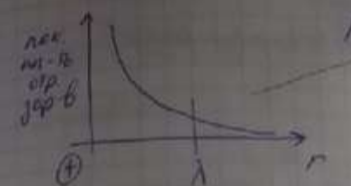
\includegraphics[width=0.6\linewidth]{lecture_09/pic8}
	
\end{figure}
	
	$l_2 = \left[\dfrac{e^2}{\varepsilon k T}\right]$ - равенство Онзагера, $l_1 = n^{-1/3}, \lambda = l_1^\alpha l_2^{1- \alpha}$. $\sqrt{\dfrac{l_1^3}{l_2}}, \lambda \sim \sqrt{\dfrac{\varepsilon k T}{n e^2}}.$
	
\end{lecSection}
			
\end{lecture}